\documentclass[border=5mm]{standalone}
\usepackage{tkz-euclide}
\usetkzobj{all}
\begin{document}
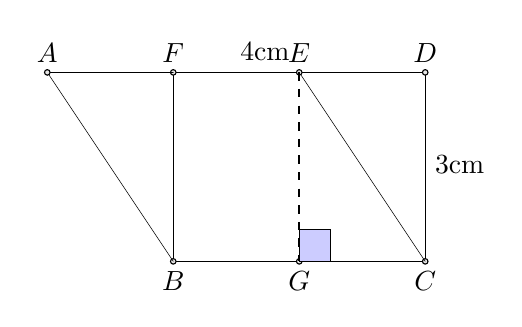
\begin{tikzpicture}[scale=.8]

\tkzDefPoint(0,0){B} \tkzDefPoint(4,0){C}
\tkzDefPoint(4,3){D} \tkzDefPoint(0,3){F}

\draw (0,0) rectangle (4,3);
\tkzDrawPoints(F,B,C,D)
\tkzLabelPoints[below](C,B)
\tkzLabelPoints[above](F,D)


\node [right] at (4,1.5) {\strut 3cm};
\node [left] at (2,3.3) {\strut 4cm};

\tkzDefPoint(2,3){E}
\tkzDefPoint(-2,3){A}
\tkzDrawSegments(E,C A,B A,F)
\tkzDrawPoints(E,A)
\tkzLabelPoints[above](E,A)

\tkzDefPoint(2,0){G}
\tkzDrawPoints(G)
\tkzLabelPoints[below](G)
\draw [thick,dashed] (E) -- (G);
\tkzMarkRightAngle[fill=blue!20,size=0.5](E,G,C)




\end{tikzpicture}
\end{document}
\grid
\grid
\grid
